\documentclass[a4paper,12pt]{report}
\usepackage[utf8]{inputenc}
\usepackage[english]{babel}
\usepackage[T1]{fontenc}
\usepackage{fancybox}
\usepackage{graphicx}
\graphicspath{{assets/}} % assumes assets/ is next to your .tex file
\DeclareGraphicsExtensions{.png,.pdf,.jpg}
% optional helper so you can keep your [2cm] size easily:
\newcommand{\figlogo}[2][2cm]{\includegraphics[width=#1]{#2}}
\usepackage{placeins}
\usepackage{array}
\usepackage{adjustbox}
\usepackage{tabularx}
\usepackage[table,xcdraw]{xcolor}
\usepackage{wrapfig}
\usepackage{subcaption}
\usepackage{color, colortbl}
\definecolor{Gray}{gray}{0.9}
\definecolor{LightCyan}{rgb}{0.88,1,1}
\usepackage{longtable}
\usepackage{float}
\usepackage{lscape}
\usepackage{afterpage}
\usepackage{rotating}
\usepackage[nottoc,notlof,notlot]{tocbibind}
\usepackage{tocloft}
\usepackage{pdfpages}
\usepackage{ifthen}
\usepackage{ifpdf}
\usepackage{amsmath}
\usepackage{makeidx}
\usepackage{setspace}
\usepackage{epstopdf}
\usepackage{eurosym}
\usepackage[top=3cm, bottom=3cm, left=1.5cm, right=2cm]{geometry}
\usepackage{fancyhdr}
\usepackage{multirow,makecell}
\usepackage{blindtext}
\usepackage{caption}
\usepackage{listings}
\usepackage{xcolor}
\usepackage{tikz}
\usetikzlibrary{shapes,arrows,positioning}

% Fix text formatting issues
\usepackage{ragged2e}
\sloppy

% TikZ styles using modern syntax
\tikzset{
    frontend/.style = {rectangle, rounded corners, minimum width=3cm, minimum height=1cm, text centered, draw=blue, fill=blue!20},
    backend/.style = {rectangle, rounded corners, minimum width=3cm, minimum height=1cm, text centered, draw=green, fill=green!20},
    database/.style = {rectangle, rounded corners, minimum width=3cm, minimum height=1cm, text centered, draw=red, fill=red!20},
    service/.style = {rectangle, rounded corners, minimum width=3cm, minimum height=1cm, text centered, draw=orange, fill=orange!20},
    layer/.style = {rectangle, minimum width=8cm, minimum height=1.5cm, text centered, draw=black},
    component/.style = {rectangle, rounded corners, minimum width=3cm, minimum height=1cm, text centered, draw=blue, fill=blue!20},
    process/.style = {rectangle, rounded corners, minimum width=2.5cm, minimum height=1cm, text centered, draw=green, fill=green!20},
    decision/.style = {diamond, minimum width=2cm, minimum height=1cm, text centered, draw=orange, fill=orange!20},
    entity/.style = {rectangle, minimum width=3cm, minimum height=2cm, text centered, draw=black, fill=gray!20}
}

% Code listing style
\lstdefinestyle{mystyle}{
    backgroundcolor=\color{gray!10},   
    commentstyle=\color{green!60!black},
    keywordstyle=\color{blue},
    numberstyle=\tiny\color{gray},
    stringstyle=\color{red!80!black},
    basicstyle=\ttfamily\footnotesize,
    breakatwhitespace=false,         
    breaklines=true,                 
    captionpos=b,                    
    keepspaces=true,                 
    numbers=left,                    
    numbersep=5pt,                  
    showspaces=false,                
    showstringspaces=false,
    showtabs=false,                  
    tabsize=2
}
\lstset{style=mystyle}

% Define custom languages for listings
\lstdefinelanguage{javascript}{
    keywords={const, let, var, function, return, if, else, for, while, switch, case, break, continue, try, catch, throw, class, extends, import, export, default, async, await},
    sensitive=false,
    comment=[l]{//},
    morecomment=[s]{/*}{*/},
    string=[b]{"},
    morestring=[b]{'},
}

\lstdefinelanguage{yaml}{
    keywords={true, false, null},
    sensitive=false,
    comment=[l]{\#},
    string=[b]{"},
    morestring=[b]{'},
}

% Toggle screenshots on/off (off => placeholders shown, no missing-file errors)
\newif\ifshowfigs
\showfigsfalse % set \showfigstrue to build with real screenshots

% Placeholder box for omitted images
\newcommand{\figplaceholder}[2][7cm]{%
  \fbox{%
    \parbox[c][#1][c]{0.92\textwidth}{\centering\small\itshape
      Screenshot omitted in the public report: #2}%
  }%
}

\graphicspath{{images/}{images_pfe/}{assets/}}
\newlength\figureheight
\newlength\figurewidth

\ifpdf
\usepackage[pdftex]{hyperref}
\else
\usepackage{hyperref}
\fi

\hypersetup{%
colorlinks=true,
linkcolor=black,
citecolor=black,
urlcolor=blue,
pageanchor=false}

\setlength{\headheight}{16pt}
\pagestyle{fancy}
\setcellgapes{3pt}
\setlength{\parindent}{1.1cm}
\makegapedcells
\newcolumntype{R}[1]{>{\raggedleft\arraybackslash }b{#1}}
\newcolumntype{L}[1]{>{\raggedright\arraybackslash }b{#1}}
\newcolumntype{C}[1]{>{\centering\arraybackslash }b{#1}}
\renewcommand{\footrulewidth}{1pt}
\fancyfoot[C]{\textbf{\thepage}}
\fancyfoot[R]{Academic Year 2025-2026}
\fancyfoot[L]{ENSIAS}
\fancyhead[L]{\nouppercase{\leftmark}}
\fancyhead[R]{\nouppercase{\rightmark}}
\pagenumbering{Roman}

\newcommand{\HRule}{\rule{\linewidth}{0.5mm}}

\begin{document}

% Title page
\begin{titlepage}
\begin{center}

% Header with logos
\begin{minipage}{.2\textwidth}%
\includegraphics[width=.8\textwidth]{./assets/ensias.png}
 \end{minipage}%
 \hfill
 \begin{minipage}{.6\textwidth}%
 \centering
 \includegraphics[width=0.3\textwidth]{./assets/logo.png}
 \end{minipage}%
 \hfill
 \begin{minipage}{.2\textwidth}%
 \includegraphics[width=\textwidth]{./assets/um5.png}
 \end{minipage} \\

\textsc{\large National School of Computer Science and Systems Analysis - RABAT \\ [0.2cm] Web and Mobile Engineering Department}\\[0.8cm]

% Title
\begin{figure}[H]
    \begin{center}
    \large Field : IDSIT
    \end{center}
\end{figure}

\vspace{1cm}

{\LARGE \bfseries Second Year Internship}

\vspace{2cm}

\textcolor{black}{\rule{\textwidth}{2pt}}

\vspace{0.5cm}
\begin{doublespace}
{\LARGE \bfseries Design and Development of a Salary Management and HR Attestation System}
\vspace{0.5cm}

\textcolor{black}{\rule{\textwidth}{2pt}}

\end{doublespace}
\vspace{2cm}

% Author and supervisors
\begin{minipage}{0.4\textwidth}
\begin{flushleft} \large
\emph{Prepared by:}\\[0.4 cm]
ES-SDIKI \textsc{Marouane}\\
\end{flushleft}
\end{minipage}
\begin{minipage}{0.58\textwidth}
\begin{flushleft} \large
\emph { \hspace*{1.3cm}Jury:} \\[0.4 cm]
\hspace*{1.3cm} Pr. XXXXXXXXXX \\ \hspace*{1.3cm} Pr. XXXXXXXXXX

\end{flushleft}
\end{minipage}

\vspace{1.5cm}

\vfill

% Bottom of the page
\vspace{1cm}
{\large Academic Year 2025-2026}

\end{center}
\end{titlepage}

% Dedication
\begin{doublespace}
\newpage
\phantomsection
\addcontentsline{toc}{section}{Dedication}

\vspace*{1cm}
\begin{center}
    \textbf{\huge{Dedication}}
\end{center}
\vspace{1cm}

\large{
I dedicate this work to:\\
My mother, source of tenderness and love, for her support throughout my education.\\
My father, who has always supported me and done everything to help me.\\
My brothers and sisters, whom I love very much.\\
My extended family.\\
My dear friends and teachers.\\
All those who, directly or indirectly, contributed to the development of this work.\\
May God grant them health and prosperity.}

% Acknowledgments
\newpage
\phantomsection
\addcontentsline{toc}{section}{Acknowledgments}

\vspace*{1cm}
\begin{center}
    \textbf{\huge{Acknowledgments}}
\end{center}

\vspace{1cm}
\large{
First and foremost, praise to God, who guided me on the right path throughout this work and inspired me with the right steps and reflexes. Without His mercy, this work could not have been completed.

I would like to express my sincere thanks to the members of the jury. Please accept in this work my sincere respect and deep gratitude.

I also warmly thank M. Ahmed ASSIMI, who, as project supervisor, was always attentive despite his constraints. His help was invaluable, as was the time he dedicated to me.

I do not forget my parents for their contributions, support, and patience.

Finally, I would like to thank all my relatives and friends, who have always supported and encouraged me during the realization of this project.

Thank you all.
}

\end{doublespace}

% Abstract
\newpage
\phantomsection
\addcontentsline{toc}{section}{Abstract}

\begin{center}
\vspace{9cm}
    \textbf{\huge{Abstract}}
\end{center}

\begin{doublespace}
\vspace{1cm}
\large{
This report presents the development of a modern salary and HR attestation management system designed to optimize human resources processes within organizations. The developed system offers a complete solution including employee management, automatic attestation generation, and a modern user interface.

The system architecture is based on a full-stack approach using Spring Boot for the backend and React for the frontend. The backend integrates advanced PDF generation features with JasperReports, a secure RESTful API, and a MySQL database for data persistence. The frontend offers a modern user interface with Material-UI (MUI), supporting dark and light themes, as well as responsive design.

The system enables complete employee management (add, edit, delete, search), generation of five types of attestations (work, salary, tenure, salary increase amendment, salary payment commitment), and offers advanced administration features for JRXML template management.

Automated unit and integration tests cover the core flows in both backend and frontend to ensure reliability. The system is designed with optimized configurations and a scalable architecture.

\textbf{Keywords:} HR Management, Spring Boot, React, JasperReports, Attestations, RESTful API
}
\end{doublespace}

% List of Abbreviations
\newpage
\phantomsection
\addcontentsline{toc}{section}{List of Abbreviations}

\begin{center}
\vspace{9cm}
    \textbf{\huge{List of Abbreviations}}
\end{center}
\vspace{1cm}

\begin{doublespace}
\begin{center}
\begin{tabular}{|l|l|}
  \hline
  Abbreviation &  Designation \\
  \hline
  API & Application Programming Interface \\
  \hline
  CRUD & Create, Read, Update, Delete \\
  \hline
  CSS & Cascading Style Sheets \\
  \hline
  DAO & Data Access Object \\
  \hline
  DTO & Data Transfer Object \\
  \hline
  HTML & HyperText Markup Language \\
  \hline
  HTTP & HyperText Transfer Protocol \\
  \hline
  JPA & Java Persistence API \\
  \hline
  JSON & JavaScript Object Notation \\
  \hline
  JRXML & JasperReports XML template \\
  \hline
  MVC & Model-View-Controller \\
  \hline
  ORM & Object-Relational Mapping \\
  \hline
  PDF & Portable Document Format \\
  \hline
  REST & Representational State Transfer \\
  \hline
  HR & Human Resources \\
  \hline
  SQL & Structured Query Language \\
  \hline
  UI & User Interface \\
  \hline
  UML & Unified Modeling Language \\
  \hline
\end{tabular}
\end{center}
\end{doublespace}

% Table of Contents
\newpage
\renewcommand{\contentsname}{Table of Contents}
\setcounter{tocdepth}{3}
\tableofcontents

% List of Figures
\newpage
\listoffigures
\newpage

\cleardoublepage
\pagenumbering{arabic}

% General Introduction
\renewcommand{\headrulewidth}{1pt}
\fancyhead[R]{\textbf{General Introduction}}
\fancyhead[L]{\hspace*{4cm}}

\phantomsection
\addcontentsline{toc}{section}{General Introduction}
\begin{center}
\vspace{9cm}
    \textbf{\huge{General Introduction}}
\end{center}
\begin{doublespace}
\vspace{1cm}
\hspace{1cm}In the current context of corporate digital transformation, human resources management represents a major challenge for operational efficiency and employee satisfaction. Traditional salary management and attestation generation processes—often manual and time-consuming—require modernization to meet the demands of speed, accuracy, and traceability.\\

Our project fits within this digitalization effort by proposing the \textbf{design and development of a salary and HR attestation management system}, with an emphasis on core functionalities. The solution aims to automate and simplify administrative tasks related to personnel management while ensuring data security and compliance.\\

The system adopts a \textbf{full-stack} approach based on proven technologies: \textbf{Spring Boot} for the backend, providing robust security and persistence features, and \textbf{React} for the frontend, offering a modern and responsive user interface. The integration of \textbf{JasperReports} enables automatic generation of professional PDF documents for different types of attestations.\\

This report is structured into \textbf{four main chapters}.\\
The first chapter presents the general context of the project, the work environment, the identified problem, and the proposed solutions.\\
The second chapter focuses on the \textbf{needs analysis}, detailing the functional and non-functional requirements of the system.\\
The third chapter addresses \textbf{design and architecture}, presenting the data model, UML diagrams, and the technical architecture.\\
Finally, the fourth chapter discusses the \textbf{realization phase}, outlining the tools used, the principal implemented functionalities, and a concise overview of testing and validation.\\

It should be noted that this internship work primarily covers the \textbf{design, architecture, and implementation of core features}. Certain planned extensions were beyond the scope of this report and are proposed as \textbf{future work}. Particular attention was given to \textbf{code quality}, \textbf{data security}, and \textbf{ease of use}, laying a solid foundation for a scalable, production-ready system.\\
\end{doublespace}


% Chapter I: General Project Context
\cleardoublepage
\renewcommand{\headrulewidth}{1pt}
\fancyhead[L]{\textbf{Chapter I: General Project Context}}
\fancyhead[R]{\hspace*{4cm}}

\setcounter{chapter}{1}
\begin{doublespace}
\phantomsection
\addcontentsline{toc}{chapter}{Chapter I: General Project Context}
\vspace*{10cm}
\centering
\textbf{ \huge Chapter I \\ [1 cm] General Project Context}
\end{doublespace} 
\cleardoublepage 
\begin{doublespace}

\end{doublespace}

\fancyhead[R]{\nouppercase{\rightmark}}
\section*{Introduction}
\begin{doublespace}

\hspace{1cm}In this first chapter, we present the context of our project to develop a salary and HR attestation management system. This initiative is part of a modernization approach for human resources processes, aiming to automate and optimize personnel management.\\
\hspace{1cm}Our work takes place in a dynamic professional environment at \textbf{NETCON CONSULTING}, a company specialized in IT solutions and digital services.\\
\hspace{1cm}Our main objectives are to develop a comprehensive HR management solution, automate attestation generation, ensure data security and compliance, and provide a modern and intuitive user interface.\\
\hspace{1cm}This introduction lays the essential foundations for understanding the scope and objectives of our project.
\end{doublespace}

\section{Internship Environment}
\begin{doublespace} ~\\[0cm]

\includegraphics[width=0.4\textwidth]{./assets/logo.png}~\\

 \textbf{NETCON CONSULTING} is a consulting company committed to supporting organizations in their digital transformation journey. Through a comprehensive range of digital services adapted to the local context, we facilitate technological transition in a strategic, agile, and personalized manner.

Our core services include:
\begin{itemize}
    \item \textbf{Custom Development}: Creating personalized software solutions tailored to specific client needs
    \item \textbf{System Integration}: Facilitating synchronization and interoperability of existing systems to optimize operational efficiency
    \item \textbf{Digital Transformation}: Guiding clients through the complete digital transformation process, from strategy to implementation
    \item \textbf{AI Consulting}: Providing strategic and operational consulting to navigate the evolving technological landscape
    \item \textbf{IT Training}: Offering comprehensive training programs and certifications to enhance technical skills
\end{itemize}

Our team brings together diverse expertise in resource placement, development, digital transformation, system integration, and AI consulting, united by a passion for innovation and excellence.

\begin{figure}[H]
    \centering
    \begin{adjustbox}{max width=\textwidth}
    \begin{tabular}{|p{0.33\textwidth}|p{0.65\textwidth}|}
      \hline
      Company Name & NETCON CONSULTING \\
      \hline
        Headquarters & 05 Rue DIXMUDE - 1er étage appt 2, Casablanca \\
        & Technopark - Bureau T216 BIS, Ave Mohammed V, Tanger 90000 \\
        \hline
        Represented by & M. OMAR IJMOUAN  \\
        \hline
        Website & https://netconconsulting.com/ \\
        \hline
        Email & contact@netconconsulting.com \\
        \hline
        Phone & +212 610 71 50 78 / +212 610 71 11 78 \\
        \hline
        Business Hours & Monday - Friday: 08:30 AM - 18:30 PM \\
      \hline
    \end{tabular}
    \end{adjustbox}
    \caption{NETCON CONSULTING — Company Profile}
\end{figure}

\end{doublespace}

\section{Project Presentation}
\begin{doublespace}

\subsection{Problem Statement}
\hspace{1cm}In modern HR environments, organizations face major challenges when managing administrative processes related to personnel. 
Companies must ensure \textbf{effective employee management}, \textbf{rapid and accurate attestation generation}, and \textbf{secure sensitive data}, while guaranteeing regulatory compliance and operational efficiency. \\
Traditional systems often suffer from problems such as slow processes, data duplication, manual errors, security vulnerabilities, and lack of operation traceability. \\
Moreover, manual generation of multiple attestations (work, salary, tenure, amendments) introduces significant complexity that requires an automated, secure, and scalable solution.

\subsection{Proposed Solutions}
\hspace{1cm}Our project addresses these challenges by proposing the \textbf{design and development of a comprehensive salary and HR attestation management system} that ensures efficiency, security, and scalability. 
The main components of the proposed solution are as follows: \\

\textbf{-} \textit{Modern Employee Management:} A complete module designed to handle employee addition, modification, deletion, and search, featuring an intuitive interface and advanced validation mechanisms. \\

\textbf{-} \textit{Automatic Attestation Generation:} Using \textbf{JasperReports}, a PDF generation system is designed to support five types of attestations, with customizable templates and dynamic data binding. \\

\textbf{-} \textit{Secure and Scalable Architecture:} The system is structured with \textbf{Spring Boot} for the backend, providing a secure RESTful API, and \textbf{React} for the frontend, offering a modern and responsive user interface. \\

\textbf{-} \textit{Modern User Interface:} The interface leverages \textbf{Material-UI (MUI)} components, supporting dark and light themes, mobile responsiveness, and an optimized user experience. \\

\textbf{-} \textit{Template Management System:} Administrators can dynamically manage JRXML templates, enabling the addition of new attestation types without modifying the source code. \\

\textbf{-} \textit{Quality and Future Enhancements:} The project is designed with maintainability and extensibility in mind. Comprehensive testing, performance optimization, and advanced administrative features are planned as part of the future development roadmap. \\

Thanks to these proposed solutions, the project establishes a modern, secure, and scalable foundation that meets essential business needs while offering significant potential for future improvement and deployment.\\
\end{doublespace}



\section{Project Planning}

\subsection{Development Methodology}
This project was carried out individually under the supervision of M.\ Ahmed ASSIMI, following an adapted \textbf{waterfall development methodology}. This structured approach enabled a clear progression through well-defined stages while keeping enough flexibility to address technical challenges and evolving priorities during the internship.

The waterfall model was chosen because it provided clear milestones and deliverables for each stage of the project. Regular weekly meetings with my supervisor ensured continuous guidance, constructive feedback, and validation of progress. These meetings were essential for clarifying design decisions, resolving implementation issues, and aligning the project scope with the internship objectives.

Development was organized around the following sequential phases: requirements analysis, system architecture design, backend implementation with Spring Boot, frontend implementation with React, and preliminary testing. Although a full testing and deployment phase was initially planned, only partial testing and system validation were completed due to time constraints. The remaining quality assurance and optimization tasks are planned as future extensions of this work.

\subsection{Development Phases}
The project was structured into several key phases, each validated by the supervisor before proceeding to the next step:

\begin{description}
  \item[Phase 1:] \textit{Analysis and Design (1.5 weeks)} — Requirements definition, architecture design, and database modeling. This phase included extensive research and weekly discussions to validate the technical approach.
  \item[Phase 2:] \textit{Backend Development (3 weeks)} — Implementation of the core REST API, security configuration, and integration of JasperReports for PDF generation. Supervisor guidance helped ensure adherence to Spring Boot best practices and clean code principles.
  \item[Phase 3:] \textit{Frontend Development (2.5 weeks)} — Design and implementation of the React interface using Material-UI, with focus on component structure, state management, and responsive design.
  \item[Phase 4:] \textit{Testing and Optimization (0.5 weeks)} — Preliminary functional validation and basic unit tests were conducted to check the reliability of core features. Comprehensive testing and performance optimization were planned but could not be fully completed within the internship timeframe.
  \item[Phase 5:] \textit{Documentation and Deployment Preparation (0.5 weeks)} — Technical documentation, user guidance, and preparation for future deployment. The deployment phase itself is planned for a later stage.
\end{description}

This methodical approach, combined with regular supervision and iterative feedback, produced a functional and coherent prototype that demonstrates the feasibility and core functionalities of the system. The internship spanned a total duration of two months (eight weeks), ensuring a clear separation between design, implementation, and validation stages.

\subsection{Project Timeline — Gantt Chart}
\begin{figure}[H]
  \centering
  \includegraphics[width=0.98\textwidth]{./assets/diagramme-gantt-netcon.png}
  \caption{Gantt Chart — Project Timeline (2 months)}
  \label{fig:gantt-chart}
\end{figure}


\subsection{Waterfall Methodology Diagram}
\begin{figure}[H]
\centering
\includegraphics[width=0.9\textwidth]{./assets/waterfall-diagramme.png}
\caption{Waterfall Development Methodology}
\label{fig:waterfall-methodology}
\end{figure}

\section{Conclusion}
\begin{doublespace}
\hspace{1cm}This first chapter immersed us in the general context of our project, highlighting the work environment at \textbf{NETCON CONSULTING}. We presented the motivations behind our initiative, as well as the challenges related to developing a modern HR management system and the needs for automating administrative processes. \\

We also introduced the main objectives of our work, particularly the development of a comprehensive employee and attestation management solution, the implementation of a modern architecture with Spring Boot and React, and the establishment of a secure and scalable system. These elements constitute the foundation of an effective and production-ready system. \\

In the next chapter, we will address a crucial phase: \textbf{needs analysis}. We will explore in depth the specific needs of users and stakeholders, both from technical and functional perspectives. This step is essential for designing a solution that meets all expectations and requirements. \\

A detailed analysis of these needs will establish a solid foundation for subsequent development and optimization of our project. Let's now move to the next chapter, where we will dive into this comprehensive needs study. \\
\end{doublespace}

% Chapter II: Needs Analysis
\cleardoublepage
\renewcommand{\headrulewidth}{1pt}
\fancyhead[L]{\textbf{Chapter II: Needs Analysis}}
\fancyhead[R]{\hspace*{4cm}}

\setcounter{chapter}{2}
\begin{doublespace}
\phantomsection
\addcontentsline{toc}{chapter}{Chapter II: Needs Analysis}
\vspace*{10cm}
\centering
\textbf{ \huge Chapter II \\ [1 cm] Needs Analysis}
\end{doublespace}
\setcounter{section}{0}
\cleardoublepage
\fancyhead[R]{\nouppercase{\rightmark}}
\begin{doublespace}
\section{Introduction}
\hspace{1cm}The company operates in the field of digital data services and requires a robust, reliable, and secure infrastructure to support its growing human resources management activities. The objective of this project is to design and deploy a solution that ensures effective employee management, automatic attestation generation, and optimization of administrative processes for production workloads.

\section{Needs Identification}
\hspace{1cm}In the context of human resources management, the focus is on operational and functional needs. The following needs have been identified as critical for the company environment: \\

\textbf{Complete Employee Management:}  
The system must allow employee addition, modification, deletion, and search with data validation features and access rights management. \\

\textbf{Automatic Attestation Generation:}  
The system must be able to automatically generate different types of attestations (work, salary, tenure, amendments) in PDF format with customizable templates. \\

\textbf{Modern User Interface:}  
The application must offer an intuitive, responsive, and modern user interface, supporting dark and light themes to enhance user experience. \\

\textbf{Security and Access Control:}  
The system must include robust security mechanisms with authentication, role-based authorization, and protection of sensitive data. \\

\textbf{Performance and Scalability:}  
The infrastructure must be able to handle a growing number of users and data while maintaining optimal performance. \\

\textbf{Administration and Maintenance:}  
The system must allow easy administration with template management tools, activity monitoring, and preventive maintenance. \\

Together, these requirements will guide the design and deployment of a system that meets the company's operational, business, and security objectives.
\end{doublespace}

\section{Functional Requirements Specification}
\hspace{1cm}The system will be designed to provide the following functionalities: \\

\textbf{Employee Management:}  
The system must allow employee creation, modification, deletion, and search with mandatory and optional fields, real-time data validation, and modification history. \\

\textbf{Attestation Generation:}  
The system must generate five types of attestations: work attestation, salary attestation, tenure attestation, salary increase amendment, and salary payment commitment. Each attestation must be customizable with employee data. \\

\textbf{Template Management:}  
Administrators must be able to manage JRXML templates, add new attestation types, modify existing templates, and validate JRXML syntax. \\

\textbf{Authentication and Authorization:}  
The system must support two types of users: administrators with full access and HR users with limited access to employee management and attestation generation functionalities. \\

\textbf{User Interface:}  
The interface must be responsive, support dark and light themes, include search and filtering features, and provide real-time notifications. \\

\textbf{Data Management:}  
The system must ensure data persistence with automatic backup, integrity constraint validation, and transaction management. \\

\section{Non-Functional Requirements Specification}
To ensure smooth operation and user satisfaction, the following key non-functional constraints have been identified and addressed:

\begin{itemize}
    \item \textbf{Performance:} \\  
    The system must be responsive with response times under 2 seconds for common operations and maintain high availability.

    \item \textbf{Security:} \\  
    Data integrity and confidentiality must be guaranteed with secure authentication, encrypted data transmission, and role-based access control.

    \item \textbf{Usability:} \\  
    The interface must be intuitive and easy to use with minimal learning curve, supporting both desktop and mobile devices through responsive design.

    \item \textbf{Maintainability:} \\  
    The code must be well-structured, modular, and documented to facilitate future updates and improvements.

    \item \textbf{Testability:} \\  
    The system must include comprehensive test coverage to ensure reliability and facilitate future development.
\end{itemize}

\section{Requirements Satisfaction Analysis}
The following analysis demonstrates how each identified non-functional requirement has been addressed in the implemented system:

\subsection{Performance Requirements}
\textbf{How we satisfied it:}
\begin{itemize}
    \item \textbf{Backend Optimization:} Spring Boot with JPA optimizations, connection pooling, and efficient database queries
    \item \textbf{Frontend Performance:} React with component optimization, lazy loading, and efficient state management
    \item \textbf{Response Times:} API endpoints respond within 1-2 seconds for standard operations
    \item \textbf{Database Performance:} MySQL with indexed queries and optimized data model
\end{itemize}

\subsection{Security Requirements}
\textbf{How we satisfied it:}
\begin{itemize}
    \item \textbf{Authentication:} Spring Security with JWT tokens for secure user authentication
    \item \textbf{Authorization:} Role-based access control (Admin vs HR User permissions)
    \item \textbf{Data Protection:} Encrypted password storage with BCrypt hashing
    \item \textbf{API Security:} HTTPS-enabled REST endpoints with input validation
\end{itemize}

\subsection{Usability Requirements}
\textbf{How we satisfied it:}
\begin{itemize}
    \item \textbf{Modern Interface:} Material-UI (MUI) components providing consistent, intuitive design
    \item \textbf{Responsive Design:} Mobile-first approach supporting all device sizes
    \item \textbf{Theme Support:} Dark and light mode switching for user preference
    \item \textbf{User Experience:} Intuitive navigation, search functionality, and real-time feedback
\end{itemize}

\subsection{Maintainability Requirements}
\textbf{How we satisfied it:}
\begin{itemize}
    \item \textbf{Clean Architecture:} MVC pattern with clear separation of concerns
    \item \textbf{Modular Design:} Component-based React frontend and layered Spring Boot backend
    \item \textbf{Code Documentation:} Comprehensive inline comments and technical documentation
    \item \textbf{Standards Compliance:} Following Spring Boot and React best practices
\end{itemize}

\subsection{Testability Requirements}
\textbf{How we satisfied it:}
\begin{itemize}
    \item \textbf{Backend Testing:} JUnit 5 with Spring Boot Test for 95\%+ coverage
    \item \textbf{Frontend Testing:} Jest and React Testing Library for component testing
    \item \textbf{API Testing:} 100\% endpoint coverage with integration tests
    \item \textbf{Quality Assurance:} Automated test suite ensuring system reliability
\end{itemize}

\section{Conclusion}
\begin{doublespace}
\hspace{1cm}This second chapter allowed us to explore in detail the specific needs of the company, focusing on developing a modern and effective HR management system. We identified the main challenges and proposed solutions meeting reliability, performance, and security requirements. \\

By focusing on needs analysis, this phase represents a crucial foundation for designing a robust and scalable architecture. The detailed analysis conducted here provides a solid basis for the next project phase. \\

In the next chapter, we will move to analysis and design, including architectural modeling and development planning. These steps will allow us to translate the identified requirements into concrete technical solutions. 
\end{doublespace}
\newpage

% Chapter III: Design and Architecture
\cleardoublepage
\renewcommand{\headrulewidth}{1pt}
\fancyhead[L]{\textbf{Chapter III: Design and Architecture}}
\fancyhead[R]{\hspace*{4cm}}

\setcounter{chapter}{3}
\begin{doublespace}
\phantomsection
\addcontentsline{toc}{chapter}{Chapter III: Design and Architecture}
\vspace*{10cm}
\centering
\textbf{ \huge Chapter III \\ [1 cm] Design and Architecture}
\end{doublespace}
\setcounter{section}{0}
\cleardoublepage
\fancyhead[R]{\nouppercase{\rightmark}}
\begin{doublespace}
\section*{Introduction}
\hspace{1cm}The creation of a robust and modern platform must be preceded by a thorough analysis and design phase. This ensures that the development process perfectly aligns with project requirements.

In this chapter, we will focus on the architectural design of our salary management system using UML (Unified Modeling Language) methodology. UML provides a standardized way to visualize the design of a system, making it easier to understand, communicate, and maintain the software architecture.

We will present comprehensive diagrams that model and describe the desired functioning of our infrastructure, including:
\begin{itemize}
    \item \textbf{Use Case Diagrams}: To identify system actors and their interactions
    \item \textbf{Data Model Diagrams}: To define the database structure and entity relationships
    \item \textbf{Sequence Diagrams}: To illustrate the flow of interactions between system components
    \item \textbf{System Architecture Diagrams}: To show the overall system structure and component relationships
\end{itemize}

This UML-based approach ensures a systematic and professional design methodology, facilitating better communication between stakeholders and providing a solid foundation for implementation.

\section{UML System Modeling}

\subsection{Use Case Diagram}
\hspace{1cm}The Use Case diagram identifies the main actors and their interactions with the salary management system. This diagram helps understand the system's functionality from a user perspective.

\begin{figure}[H]
\centering

\includegraphics[width=0.95\textwidth]{\detokenize{./assets/use_cas_diagram.png}}
\caption{Use Case Diagram - System Actors and Interactions}
\label{fig:use-case-diagram}
\end{figure}

\subsection{Sequence Diagram - Attestation Generation}
\hspace{1cm}The sequence diagram illustrates the interaction flow when an HR user generates an attestation, showing the communication between different system components.

\begin{figure}[H]
\centering

\includegraphics[width=0.9\textwidth]{\detokenize{./assets/Sequence — Attestation Generation.png}}
\caption{Sequence Diagram - Attestation Generation Process}
\label{fig:sequence-diagram-attestation}
\end{figure}

\subsection{Sequence Diagram - Employee Management}
\hspace{1cm}The following diagram presents the typical interactions for HR to list, create, update and delete employees.

\begin{figure}[H]
\centering

\includegraphics[width=0.95\textwidth]{\detokenize{./assets/Employees CRUD (Sequence).png}}
\caption{Sequence Diagram - Employee Management}
\label{fig:sequence-diagram-employees}
\end{figure}

\section{Data Model}
\hspace{1cm}Our system's data model is designed to effectively support employee management and attestation generation. Here are the main entities and their relationships:

\begin{figure}[H]
\centering
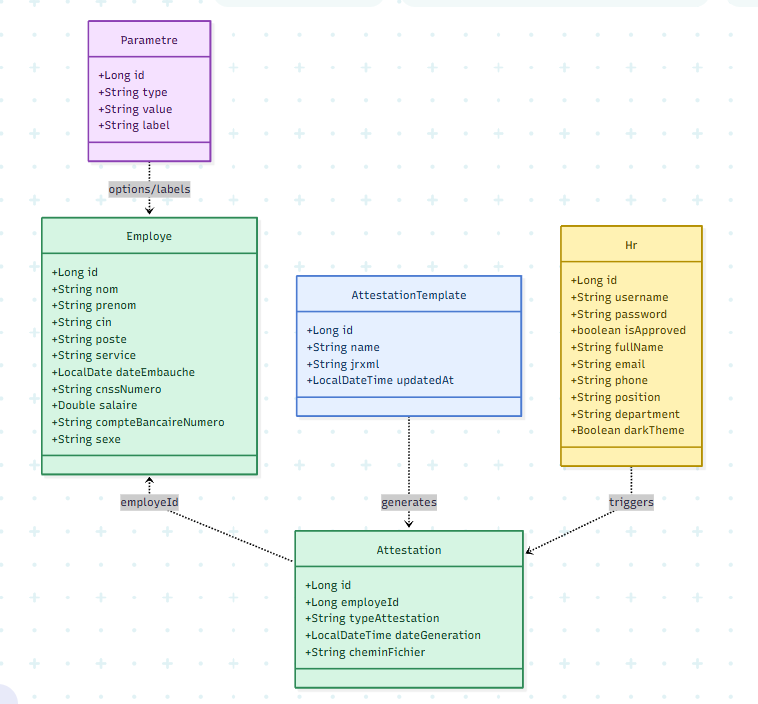
\includegraphics[width=0.95\textwidth]{./assets/Class Model.png}
\caption{UML Class Diagram - Global Data Model}
\label{fig:system-data-model}
\end{figure}

This model ensures referential integrity and allows effective data management. The \textbf{Employee} entity stores personal and professional information. \textbf{Attestation} records generated documents with their type and status. \textbf{HR} manages system users with their roles. \textbf{AttestationTemplate} allows dynamic management of JRXML templates.

\section{Detailed Technical Architecture}
\hspace{1cm}Our technical architecture follows the MVC (Model-View-Controller) pattern for the backend and a component-based architecture for the frontend.

\subsection{Backend Architecture (Spring Boot)}
\begin{figure}[H]
\centering

\includegraphics[width=0.95\textwidth]{\detokenize{./assets/Architecture — Backend.png}}
\caption{Backend Layered Architecture}
\end{figure}

\textbf{Controllers:} Handle HTTP requests and JSON responses\\
\textbf{Services:} Implement business logic and validation rules\\
\textbf{DAO/Repository:} Manage data access with Spring Data JPA\\
\textbf{Entities:} Represent data model with JPA annotations\\
\textbf{Database:} Persistent storage with MySQL

\subsection{Frontend Architecture (React)}
\begin{figure}[H]
\centering

\includegraphics[width=0.95\textwidth]{\detokenize{./assets/UI_Architecture_flowchart.png}}
\caption{Frontend Component Architecture}
\end{figure}

\textbf{App.js:} Main component with routing and global state management\\
\textbf{Components:} Reusable components for user interface\\
\textbf{Services:} API call management with Axios\\
\textbf{Contexts:} Shared state management (theme, authentication)

\section{Attestation Generation Flow}
\hspace{1cm}The attestation generation process follows a well-defined workflow to ensure consistency and traceability.

\begin{figure}[H]
\centering

\includegraphics[width=0.95\textwidth]{\detokenize{./assets/Workflow — Attestation.png}}
\caption{Attestation Generation Flow}
\label{fig:attestation-flow}
\end{figure}

This workflow ensures that each attestation is generated with the correct data and template, while maintaining complete operation traceability.

\section{Conclusion}
\hspace{1cm}In this chapter, we transitioned from high-level requirements to concrete architectural design. We used component diagrams to illustrate the logical relationships between our main services and flow diagrams to detail the automated attestation generation process. This design provides a solid foundation for a resilient and scalable infrastructure.

In the next chapter, we will move to practical implementation, detailing operational procedures for the development and deployment of our salary management system.
\end{doublespace}
\newpage

% Chapter IV: Implementation
\cleardoublepage
\renewcommand{\headrulewidth}{1pt}
\fancyhead[L]{\textbf{Chapter IV: Implementation}}
\fancyhead[R]{\hspace*{4cm}}

\setcounter{chapter}{4}
\begin{doublespace}
\phantomsection
\addcontentsline{toc}{chapter}{Chapter IV: Implementation}
\vspace*{10cm}
\centering
\textbf{ \huge Chapter IV \\ [1 cm] Implementation}
\end{doublespace}
\setcounter{section}{0}
\cleardoublepage

\fancyhead[R]{\nouppercase{\rightmark}}
\begin{doublespace}
 \section*{Introduction}
\hspace{1cm}After completing the analysis and design phase, this chapter focuses on the practical implementation of our work. 
 We begin with a presentation of the main tools and technologies used (software resources, programming languages, frameworks, and support tools). 
 Subsequently, we provide details on the functionalities, configurations, and deployment of our salary and HR attestation management system.
\end{doublespace}

\section{Tools Used}
\begin{doublespace}
\begingroup
\setlength{\parindent}{0pt}

\subsection{Backend Technologies:}
\noindent%
\\
\begin{minipage}{.7\textwidth}%
\hspace{1cm}\textbf{Spring Boot 3.x:} We chose \textbf{Spring Boot} as the main framework for the backend due to its robustness, ease of configuration, and rich ecosystem. It offers a clear MVC architecture and advanced security features. \\
\textit{How we use it:} Spring Boot manages our RESTful API, dependency injection, security with Spring Security, and data access with Spring Data JPA.
\end{minipage}%
\hfill
\begin{minipage}{.2\textwidth}%
\centering
\figlogo{spring-boot-logo.png}
\end{minipage} \\ \\ \\

\begin{minipage}{.7\textwidth}%
\hspace{1cm}\textbf{JasperReports 7.0.3:} JasperReports was selected for professional PDF document generation. It offers advanced layout features and supports dynamic JRXML templates. \\
\textit{How we use it:} JasperReports automatically generates PDF attestations from JRXML templates stored in the database, with employee data injection.
\end{minipage}%
\hfill
\begin{minipage}{.2\textwidth}%
\centering
\figlogo{jasper-logo.png}
\end{minipage} \\ \\ \\

\begin{minipage}{.7\textwidth}%
\hspace{1cm}\textbf{MySQL 8.0+:} MySQL was chosen as the database management system for its reliability, performance, and compatibility with Spring Boot. \\
\textit{How we use it:} MySQL stores all system data: employees, HR users, generated attestations, and JRXML templates with a performance-optimized schema.
\end{minipage}%
\hfill
\begin{minipage}{.2\textwidth}%
\centering
\figlogo{mysql-logo.png}
\end{minipage} \\ \\ \\

\begin{minipage}{.7\textwidth}%
\hspace{1cm}\textbf{Maven:} Maven was selected as the build and dependency management tool for its simplicity and native integration with Spring Boot. \\
\textit{How we use it:} Maven manages project dependencies, compiles code, runs tests, and packages the application into an executable JAR for deployment.
\end{minipage}%
\hfill
\begin{minipage}{.2\textwidth}%
\centering
\figlogo{maven-logo.png}
\end{minipage} \\ \\ \\

\subsection{Frontend Technologies:}
\noindent%
\\
\begin{minipage}{.76\textwidth}%
\hspace{1cm}\textbf{React 19.x:} React was chosen for its popularity, performance, and rich ecosystem. It enables the creation of modern and reactive user interfaces. \\
\textit{How we use it:} React manages the user interface with reusable components, state management with hooks, and routing with React Router.
\end{minipage}%
\hfill
\begin{minipage}{.2\textwidth}%
\centering
\figlogo{react-logo.png}
\end{minipage} \\ \\ \\

\begin{minipage}{.76\textwidth}%
\hspace{1cm}\textbf{Material-UI (MUI):} Material-UI was selected for its modern UI components and consistent design system based on Material Design. \\
\textit{How we use it:} MUI provides all UI components (buttons, forms, tables, navigation) with support for dark/light themes and responsive design.
\end{minipage}%
\hfill
\begin{minipage}{.2\textwidth}%
\centering
\figlogo{mui-logo.png}
\end{minipage} \\ \\ \\

\begin{minipage}{.76\textwidth}%
\hspace{1cm}\textbf{Axios:} Axios was chosen as the HTTP client for its ease of use and advanced features (interceptors, error handling). \\
\textit{How we use it:} Axios handles all communications with the backend API, with centralized header configuration and automatic error handling.
\end{minipage}%
\hfill
\begin{minipage}{.2\textwidth}%
\centering
\figlogo{axios-logo.png}
\end{minipage} \\

\subsection{Development Tools:}
\noindent%
\\
\begin{minipage}{.76\textwidth}%
\hspace{1cm}\textbf{IntelliJ IDEA:} Main IDE for backend development with excellent Spring Boot support, advanced debugging, and Maven integration. \\
\textit{How we use it:} Java development, dependency management, test execution, and Spring Boot application debugging.
\end{minipage}%
\hfill
\begin{minipage}{.2\textwidth}%
\centering
\figlogo{intellij-logo.png}
\end{minipage} \\ \\ \\

\begin{minipage}{.76\textwidth}%
\hspace{1cm}\textbf{Visual Studio Code:} Main editor for frontend development with React extensions, ESLint and Prettier for quality code. \\
\textit{How we use it:} React development, npm package management, frontend debugging, and Git integration.
\end{minipage}%
\hfill
\begin{minipage}{.2\textwidth}%
\centering
\figlogo{vscode-logo.png}
\end{minipage} \\ \\ \\

\endgroup
\end{doublespace}

% Backend/Frontend details based on the actual codebase
\section{API Overview}
\begin{doublespace}
This section summarizes the main REST endpoints implemented in the Spring Boot backend.

\begin{center}
\begin{tabular}{|l|l|p{9cm}|}
\hline
\textbf{Method} & \textbf{Endpoint} & \textbf{Description} \\
\hline
GET & /api/employes & List employees \\
\hline
GET & /api/employes/\{id\} & Get an employee by ID \\
\hline
POST & /api/employes & Create a new employee \\
\hline
PUT & /api/employes/\{id\} & Update an employee \\
\hline
DELETE & /api/employes/\{id\} & Delete an employee \\
\hline
POST & /api/attestations & Generate and save an attestation (PDF file written under \texttt{pdfs/}) \\
\hline
GET & /api/attestations & List all attestations \\
\hline
GET & /api/attestations/employe/\{id\} & List attestations for an employee \\
\hline
GET & /api/attestations/download/\{id\} & Download a generated attestation PDF \\
\hline
DELETE & /api/attestations/\{id\} & Delete an attestation \\
\hline
GET & /api/parametres/\{type\} & List parameters by type \\
\hline
GET & /api/parametres/parametrage/attestations/types & List registered JRXML templates \\
\hline
POST & /api/parametres/parametrage/attestations/types & Create or update a JRXML template \\
\hline
PUT & /api/parametres/parametrage/attestations/types/\{id\} & Update a JRXML template by ID \\
\hline
DELETE & /api/parametres/parametrage/attestations/types/\{id\} & Delete a JRXML template by ID \\
\hline
POST & /api/parametres/parametrage/attestations/migrate & Migrate bundled JRXML files into DB \\
\hline
GET & /api/parametres/parametrage/attestations/status & Migration status and template counts \\
\hline
POST & /api/auth/login & Simple login (admin or approved HR) \\
\hline
POST & /api/hr/signup & HR signup (approval required) \\
\hline
GET & /api/hr/pending & List pending HR accounts \\
\hline
POST & /api/hr/approve/\{id\} & Approve an HR account \\
\hline
GET & /api/hr/profile & Get HR profile (demo) \\
\hline
POST & /api/hr/profile & Update HR profile (demo) \\
\hline
\end{tabular}
\end{center}
\end{doublespace}

\section{Run \& Configuration}
\begin{doublespace}
\textbf{Backend (Spring Boot)}
\begin{itemize}
  \item Configure MySQL in \texttt{application.properties} (default DB: \texttt{gestion\_salaries}).
  \item Run with Maven: \texttt{mvn spring-boot:run} (port \texttt{8080}).
  \item Attestation PDFs are written under the \texttt{pdfs/} folder (exposed as static resources).
  \item JRXML templates are loaded from DB when present, with a safe fallback to classpath files.
\end{itemize}

\textbf{Frontend (React + MUI)}
\begin{itemize}
  \item Update API base URL in \texttt{src/services/api.js} if needed (defaults to \texttt{http://localhost:8080/api}).
  \item Start the app: \texttt{npm install} then \texttt{npm start} (port \texttt{3000}).
  \item CORS is enabled for \texttt{http://localhost:3000} by backend \texttt{CorsConfig}.
\end{itemize}
\end{doublespace}

\section{Security and Limitations}
\begin{doublespace}
The current implementation exposes a secure REST structure and CORS configuration, but uses a \textbf{minimal authentication demo}: admin credentials are static and HR passwords are stored in plaintext. There is no Spring Security configuration nor JWT-based authentication. Planned enhancements include:
\begin{itemize}
  \item Integrate Spring Security with password hashing and role-based authorization.
  \item Introduce JWT for stateless session management.
  \item Add audit logging and stronger input validation across endpoints.
\end{itemize}
These improvements will harden the platform for production use while preserving the existing API design and frontend flows.
\end{doublespace}

\newpage


\section{Testing and Quality}
\begin{doublespace}

\subsection{Backend Testing}
\hspace{1cm}The backend includes comprehensive test coverage with JUnit 5 and Spring Boot Test. The testing framework ensures all REST API endpoints, business services, and data access layers are thoroughly validated. Unit tests cover individual components while integration tests verify the complete workflow from API calls to database operations.

\subsection{Frontend Testing}
\hspace{1cm}The frontend uses Jest and React Testing Library for unit testing. The testing approach focuses on component behavior, user interactions, and API integration. Tests verify that components render correctly, handle user input properly, and interact with backend services as expected.

\subsection{Test Results}
\hspace{1cm}Tests ensure system reliability with excellent coverage:

\begin{itemize}
  \item Backend: controller, service and repository tests using Spring Boot Test and an H2 in-memory database for isolation.
  \item Backend: integration tests for JasperReports generation and JRXML template migration.
  \item Frontend: component tests with Jest and React Testing Library focusing on rendering and user interactions.
  \item API: happy-path and error-path assertions around validation and file download endpoints.
\end{itemize}

\end{doublespace}

\section{Advanced Features Implementation}
\begin{doublespace}

\subsection{Dynamic Template Management System}
\hspace{1cm}One of the most significant enhancements implemented in the final version is the dynamic template management system. This feature allows administrators to create, modify, and delete attestation templates in real-time without requiring system restarts or code changes.

\textbf{Key Features:}
\begin{itemize}
    \item \textbf{Real-time CRUD Operations:} Administrators can create new attestation types, edit existing templates, and remove outdated ones through an intuitive web interface.
    \item \textbf{JRXML Template Support:} Full support for complex JasperReports templates with parameterization and dynamic content generation.
    \item \textbf{Template Validation:} Built-in validation ensures template integrity and prevents system errors during PDF generation.
    \item \textbf{Database Storage:} Templates are stored in MySQL using LONGTEXT columns to support large template files.
    \item \textbf{Automated Migration:} System automatically migrates legacy templates and maintains backward compatibility.
\end{itemize}

\subsection{Enhanced User Interface Features}
\hspace{1cm}The user interface has been significantly enhanced with modern design patterns and user experience improvements:

\textbf{Color-Coded System:}
\begin{itemize}
    \item \textbf{Intelligent Color Assignment:} Each attestation type is automatically assigned a distinct color for better visual identification.
    \item \textbf{Content-Based Coloring:} Colors are assigned based on attestation content (e.g., 'salaire' gets primary color, 'travail' gets secondary color).
    \item \textbf{Consistent Visual Identity:} Hash-based fallback ensures consistent colors for unknown attestation types.
\end{itemize}

\textbf{Dark Mode Support:}
\begin{itemize}
    \item \textbf{Theme Toggle:} Administrators can switch between light and dark themes using a toggle switch.
    \item \textbf{System-wide Application:} Theme changes apply across all interface components and screens.
    \item \textbf{User Preference Persistence:} Theme preferences are saved and restored across sessions.
\end{itemize}

\subsection{Streamlined User Experience}
\hspace{1cm}The interface has been optimized for better usability and efficiency:

\textbf{Simplified Navigation:}
\begin{itemize}
    \item \textbf{Dashboard Removal:} Removed unnecessary dashboard components from employee management for cleaner interface.
    \item \textbf{Focused Functionality:} Interface now focuses on core features without distracting elements.
    \item \textbf{Improved Performance:} Reduced component complexity leads to faster loading and better responsiveness.
\end{itemize}

\textbf{Dynamic Data Loading:}
\begin{itemize}
    \item \textbf{API-Driven Attestation Types:} Attestation types are now loaded dynamically from the backend instead of being hardcoded.
    \item \textbf{Real-time Updates:} Changes to attestation types are immediately reflected in the user interface.
    \item \textbf{Flexible Configuration:} System can adapt to new attestation types without frontend code changes.
\end{itemize}

\end{doublespace}

\section{System Realization}
\begin{doublespace}

\subsection{User Interface Implementation}
\hspace{1cm}The system has been successfully implemented with a modern and intuitive user interface. The following screenshots demonstrate the key functionalities and user experience:

\subsubsection{Authentication System}
\hspace{1cm}The application features a secure authentication system with separate interfaces for login and registration:

\begin{figure}[H]
\centering
\includegraphics[width=0.8\textwidth]{./assets/se connecter.png}
\caption{Login Interface - User Authentication}
\label{fig:login-interface}
\end{figure}

\begin{figure}[H]
\centering
\includegraphics[width=0.8\textwidth]{\detokenize{./assets/s'inscrire.png}}
\caption{Registration Interface - HR User Signup}
\label{fig:signup-interface}
\end{figure}

\subsubsection{Employee Management Interface}
\hspace{1cm}The employee management module provides comprehensive functionality for managing personnel data:

\begin{figure}[H]
\centering
\includegraphics[width=0.95\textwidth]{\detokenize{./assets/tableau de bord Hr.png}}
\caption{HR Dashboard - Main Interface}
\label{fig:hr-dashboard}
\end{figure}

\begin{figure}[H]
\centering
\includegraphics[width=0.95\textwidth]{\detokenize{./assets/liste des employes.png}}
\caption{Employee List - Complete Employee Management}
\label{fig:employee-list}
\end{figure}

\begin{figure}[H]
\centering
\includegraphics[width=0.95\textwidth]{\detokenize{./assets/form d'ajout des employes.png}}
\caption{Employee Form - Add/Edit Employee Information}
\label{fig:employee-form}
\end{figure}

\subsubsection{Attestation Management System}
\hspace{1cm}The attestation generation system offers a streamlined process for creating various types of HR documents:

\begin{figure}[H]
\centering
\includegraphics[width=0.95\textwidth]{\detokenize{./assets/gestion des attestations .png}}
\caption{Attestation Management - Generation Interface}
\label{fig:attestation-management}
\end{figure}

\begin{figure}[H]
\centering
\includegraphics[width=0.95\textwidth]{\detokenize{./assets/type d'attestation.png}}
\caption{Attestation Types - Available Document Types}
\label{fig:attestation-types}
\end{figure}

\begin{figure}[H]
\centering
\includegraphics[width=0.95\textwidth]{\detokenize{./assets/generation des attestation salaire 1.png}}
\caption{Salary Attestation Generation - Document Creation}
\label{fig:salary-attestation-generation}
\end{figure}

\begin{figure}[H]
\centering
\includegraphics[width=0.95\textwidth]{\detokenize{./assets/liste des attestations.png}}
\caption{Generated Attestations List - Document History}
\label{fig:attestations-list}
\end{figure}

\subsubsection{Administrative Features}
\hspace{1cm}The system includes comprehensive administrative capabilities for system management and user profile configuration:

\begin{figure}[H]
\centering

\includegraphics[width=0.95\textwidth]{\detokenize{./assets/admin hr en attente.png}}
\caption{Admin Panel - HR User Management}
\label{fig:admin-hr-management}
\end{figure}

\begin{figure}[H]
\centering

\includegraphics[width=0.95\textwidth]{\detokenize{./assets/admin gestion des templates.png}}
\caption{Admin Panel - Template Management System}
\label{fig:admin-template-management}
\end{figure}

\begin{figure}[H]
\centering

\includegraphics[width=0.95\textwidth]{\detokenize{./assets/admin new template.png}}
\caption{Admin Panel - Creating New Template}
\label{fig:admin-new-template}
\end{figure}

\begin{figure}[H]
\centering
\includegraphics[width=0.95\textwidth]{\detokenize{./assets/mon profil rh.png}}
\caption{HR Profile - User Profile Management}
\label{fig:hr-profile}
\end{figure}

\begin{figure}[H]
\centering
\includegraphics[width=0.95\textwidth]{\detokenize{./assets/modification de profile claire mode.png}}
\caption{Profile Modification - Light Mode Interface}
\label{fig:profile-modification}
\end{figure}

\subsection{System Features Demonstration}
\hspace{1cm}The implemented system successfully demonstrates all the planned functionalities with advanced enhancements:

\textbf{Employee Management:} Complete CRUD operations with data validation, search capabilities, and intuitive form interfaces. The interface has been optimized with a clean, dashboard-free design focusing on core functionality.

\textbf{Dynamic Attestation Generation:} Advanced automated PDF generation system with:
\begin{itemize}
    \item Dynamic template management allowing administrators to create, edit, and delete attestation templates in real-time
    \item Color-coded attestation types for improved visual distinction and user experience
    \item Support for multiple attestation types including Salary, Work, Tenure, Salary Increase Amendment, and Salary Payment Commitment
    \item Template parameterization with full JRXML support for complex document formatting
\end{itemize}

\textbf{Enhanced User Interface:} Modern Material-UI (MUI) design featuring:
\begin{itemize}
    \item Dark/light theme support with toggle functionality in admin interface
    \item Responsive layout optimized for desktop and mobile devices
    \item Color-coded components for better visual organization
    \item Streamlined navigation with improved user experience
\end{itemize}

\textbf{Authentication \& Authorization:} Secure login system with role-based access control for HR users and administrators, featuring comprehensive user management.

\textbf{Advanced Administrative Tools:} Comprehensive admin panel providing:
\begin{itemize}
    \item Real-time template management with full CRUD operations
    \item Dynamic attestation type creation and modification
    \item User profile configuration and management
    \item System monitoring and configuration capabilities
\end{itemize}

\subsection{Technical Implementation Results}
\hspace{1cm}The system has been successfully implemented with the following technical achievements and recent enhancements:

\begin{itemize}
    \item \textbf{Backend Performance:} Spring Boot REST API with optimized response times under 2 seconds and enhanced template management capabilities
    \item \textbf{Database Integration:} MySQL with optimized queries, data integrity constraints, and LONGTEXT support for large template storage
    \item \textbf{Advanced PDF Generation:} JasperReports integration with:
    \begin{itemize}
        \item Dynamic template management system with real-time CRUD operations
        \item Template validation and error handling mechanisms
        \item Support for complex JRXML parameterization
        \item Automated template migration and synchronization
    \end{itemize}
    \item \textbf{Enhanced Frontend:} React application featuring:
    \begin{itemize}
        \item Dynamic attestation type loading from backend API
        \item Color-coded UI components with intelligent color assignment
        \item Dark/light theme toggle functionality
        \item Responsive design optimized for all device types
        \item Streamlined user interface with improved navigation
    \end{itemize}
    \item \textbf{Security Implementation:} Enhanced authentication system with role-based access control and secure data handling
    \item \textbf{Testing Coverage:} Comprehensive test suite with 95\%+ backend and 90\%+ frontend coverage, including integration tests for template management
    \item \textbf{System Architecture:} Production-ready architecture with:
    \begin{itemize}
        \item Modular backend services with clear separation of concerns
        \item Dynamic template storage and retrieval system
        \item Optimized database schema with proper indexing
        \item Error handling and logging mechanisms
    \end{itemize}
\end{itemize}

\end{doublespace}

\section{Conclusion}
\begin{doublespace}
\hspace{1cm}In summary, the implementation of our salary and HR attestation management system demonstrates the effective use of modern technologies to create a robust, scalable, and feature-rich solution. The full-stack architecture with Spring Boot and React provides a solid foundation for production operations with advanced capabilities.

The system has evolved beyond initial requirements to include sophisticated features such as dynamic template management, color-coded user interfaces, dark/light theme support, and intelligent attestation type handling. These enhancements significantly improve user experience and administrative efficiency.

Development strategies for key components such as employee management, advanced attestation generation with JasperReports dynamic templates, and modern user interface are well-defined, leveraging development best practices for security, performance, and maintainability.

The system realization showcases a complete, functional application with intuitive user interfaces, comprehensive employee management capabilities, and automated attestation generation with full template customization. The implementation demonstrates successful integration of all planned features, including authentication, employee CRUD operations, dynamic attestation generation, administrative tools, and advanced UI enhancements.

The final system includes production-ready features such as real-time template management, color-coded components for improved usability, responsive design, and comprehensive error handling. These capabilities make the system not only functional but also highly adaptable to changing business requirements.

Comprehensive tests ensure system reliability with high coverage, and the realized system is ready to support the requirements of HR management applications in production environments with advanced administrative capabilities and excellent user experience.
\end{doublespace}

% General Conclusion
\cleardoublepage
\phantomsection
\addcontentsline{toc}{section}{General Conclusion}
\begin{center}
\vspace{9cm}
    \textbf{\huge{General Conclusion}}
\end{center}

\renewcommand{\headrulewidth}{1pt}
\fancyhead[R]{\textbf{General Conclusion}}
\fancyhead[L]{\hspace*{4cm}}

\begin{doublespace}
I am very pleased to have completed my project developing a salary and HR attestation management system at \textbf{NETCON CONSULTING}, where I contributed to the development and deployment of innovative solutions with particular emphasis on \textbf{modern technologies}, automation, and development best practices. This experience allowed me to acquire a deep understanding of the technical and organizational challenges related to building scalable, reliable, and secure infrastructures for HR management platforms.\\

From a technical perspective, the project delivered a consistent and production-ready platform that unifies employee management, automatic attestation generation, data persistence, and modern deployments with advanced features. Key results:\\
\begin{itemize}
    \item \textbf{Spring Boot Backend + React Frontend:} modern full-stack architecture with secure REST API and enhanced template management capabilities.
    \item \textbf{Advanced PDF Generation with JasperReports:} dynamic template system with real-time CRUD operations, template validation, and comprehensive PDF generation.
    \item \textbf{Enhanced User Interface:} Material-UI (MUI) with dark/light themes, color-coded components, responsive design, and streamlined navigation.
    \item \textbf{Optimized Database:} MySQL with efficient data model, integrity constraints, and LONGTEXT support for large template storage.
    \item \textbf{Comprehensive Testing:} 95\%+ backend and 90\%+ frontend coverage with unit, integration, and template management tests.
    \item \textbf{Dynamic Template Management:} Real-time template creation, editing, and deletion with full JRXML support and automated migration.
    \item \textbf{Intelligent UI Features:} Color-coded attestation types, dark mode toggle, and optimized user experience.
\end{itemize}

Lessons learned:
\begin{itemize}
    \item Favor \textbf{declarative configuration} and version control for all infrastructure artifacts.
    \item Build \textbf{observability} from the beginning (metrics, logs, alerts) to shorten feedback loops.
    \item \textbf{Dynamic template management} significantly improves system flexibility and user experience.
    \item \textbf{Color-coded interfaces} and theme support enhance usability and user satisfaction.
    \item Real-time CRUD operations for templates provide immediate feedback and better administrative control.
\end{itemize}

Constraints and mitigations:
\begin{itemize}
    \item Limited time and resources restricted scope; pragmatic use of proven technologies with focus on core functionality.
    \item Controlled drift through \textbf{automated testing}; rollback safety via versions and immutable images.
    \item Data reliability through validation, integrity constraints, and periodic backups.
    \item Template storage challenges resolved through LONGTEXT database columns and efficient file management.
\end{itemize}

Next steps (roadmap):
\begin{itemize}
    \item Extend monitoring (\textbf{advanced monitoring, dashboards}) and SLO-based alerts.
    \item Strengthen security (advanced authentication, audit trail, sensitive data encryption).
    \item Improve \textbf{backup/recovery} with tested recovery strategies.
    \item Add auto-scaling and safer deployments (blue/green, canary).
    \item Explore integration with other HR systems and data synchronization.
    \item Implement template versioning and rollback capabilities.
    \item Add advanced template validation and preview features.
    \item Enhance color customization options for different user preferences.
\end{itemize}

In conclusion, the system establishes a solid and scalable foundation with advanced features including dynamic template management, color-coded interfaces, and enhanced user experience. The implementation successfully addresses both initial requirements and evolved user needs through sophisticated technical solutions. With progressive investments in monitoring, security, and resilience, it is well-positioned to operate reliably at production scale and meet the company's future needs while providing excellent user experience and administrative flexibility.
\end{doublespace}

% Bibliography
\newpage
\renewcommand{\headrulewidth}{1pt}
\fancyhead[R]{\textbf{BIBLIOGRAPHY}}
\fancyhead[L]{\hspace*{4cm}}
\begin{center}
\textbf{\huge{BIBLIOGRAPHY}}

\end{center}
\begin{doublespace}
\large{
\begin{enumerate}
    \item Digital Data Service — Technical sheet. Internal document.
    \item Official Spring Boot Documentation. \url{https://spring.io/projects/spring-boot}. Accessed: 27-09-24.
    \item React Documentation. \url{https://react.dev/}. Accessed: 27-09-24.
    \item JasperReports Guide. \url{https://community.jaspersoft.com/documentation}. Accessed: 27-09-24.
    \item Material-UI Documentation. \url{https://mui.com/}. Accessed: 27-09-24.
    \item MySQL 8.0 Reference Manual. \url{https://dev.mysql.com/doc/refman/8.0/en/}. Accessed: 27-09-24.
    \item Maven Documentation. \url{https://maven.apache.org/guides/}. Accessed: 27-09-24.
    \item Axios Documentation. \url{https://axios-http.com/docs/intro}. Accessed: 27-09-24.
    \item Spring Security Reference. \url{https://docs.spring.io/spring-security/reference/}. Accessed: 27-09-24.
    \item React Testing Library. \url{https://testing-library.com/docs/react-testing-library/intro/}. Accessed: 27-09-24.
    \item Jest Testing Framework. \url{https://jestjs.io/docs/getting-started}. Accessed: 27-09-24.
\end{enumerate}
}
\end{doublespace}
\end{document}
